
\documentclass[a4paper,14pt,oneside,pdflatex,english,final,twocolumn]{article}

\usepackage[utf8]{inputenc}
\usepackage{parallel}
\usepackage{siunitx}
\usepackage{booktabs}
\usepackage{fancyhdr}
\usepackage{pdfpages} 

\usepackage[export]{adjustbox}
\usepackage[margin=0.5in]{geometry}
\addtolength{\topmargin}{0in}

\usepackage{libertine}
\renewcommand*\familydefault{\sfdefault}  %% Only if the base font of the document is to be sans serif
\usepackage[T1]{fontenc}

\title{ATX Power Supply splitter for Raspberry Pi Clusters}
\author{semaf}
\date{August 2020}

\begin{document}

\pagestyle{fancy}

\lhead{Semaf Electronics}
\chead {\today}
\rhead{bune3}

\onecolumn

\begin{figure}
	\begin{minipage}{0.47\textwidth}
		\centering
		
\includegraphics[width=.7\textwidth,left,]{img/semaf_logo.png}

	\end{minipage}
	\hfill
	\begin{minipage}{0.47\textwidth}
		\raggedleft
		\Huge \textbf{ATX Power Supply splitter for Raspberry Pi Clusters}
	\end{minipage}
\end{figure}


\begin{figure}
	\begin{minipage}{0.47\textwidth}

		\section{Overview}
		\begin{itemize}
			\item 8x USB-A port for 5V output
			\item Voltage, Current and power measurement for each channel
			\item 2x 5V output for general purposes
			\item 2x 12V output for general purposes
			\item 2x FAN connector
		\end{itemize}


	\end{minipage}
	\hfill
	\begin{minipage}{0.47\textwidth}
		\centering
		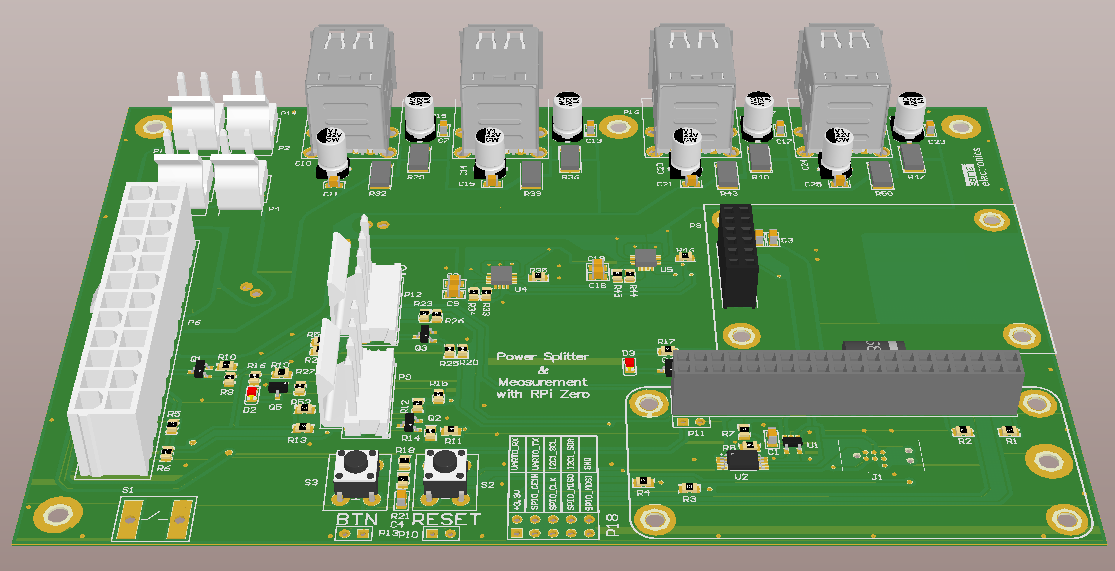
\includegraphics[width=1.0\textwidth,right]{img/Alt_Front.png}

	\end{minipage}
\end{figure}



\section{Description}
\begin{itemize}

	\item The ATX power splitter connector utilizes ATX power to split the power to 8 USB port for Raspberry Pi cluster applications.
	\item 40-pin header connector for Raspberry Pi Zero. Voltage, current and power measurement for each channel are on I²C bus available. Pi Zero is powered by 5V Standby current from ATX power supply.
	\item 2x 4-pin FAN connector, controlled by Raspberry Pi with PWM. FAN RPMs are also available for Reaspberry Pi to read. 
	\item One user button and one user LED are available for user programming. Button can be programmed as on/off switch for ATX power supply.
	\item 2x PAC1934 voltage and current sensors from microchip on I²C bus. Linux kernel driver and device tree blob are available. Device I²C addresses: 0x10, 0x1F
	\item 12-pin connector for Ethernet over SPI modules to bring the ethernet functionality to Raspberry Pi, if needed.
	\item Onboard EEPROM for board specific data as well as for HAT (Hardware Attached on Top) specifications.
	\item 10-pin header for UART, I²C, SPI connections.
	\item 
\end{itemize}

\section{Technical specification}
\noindent
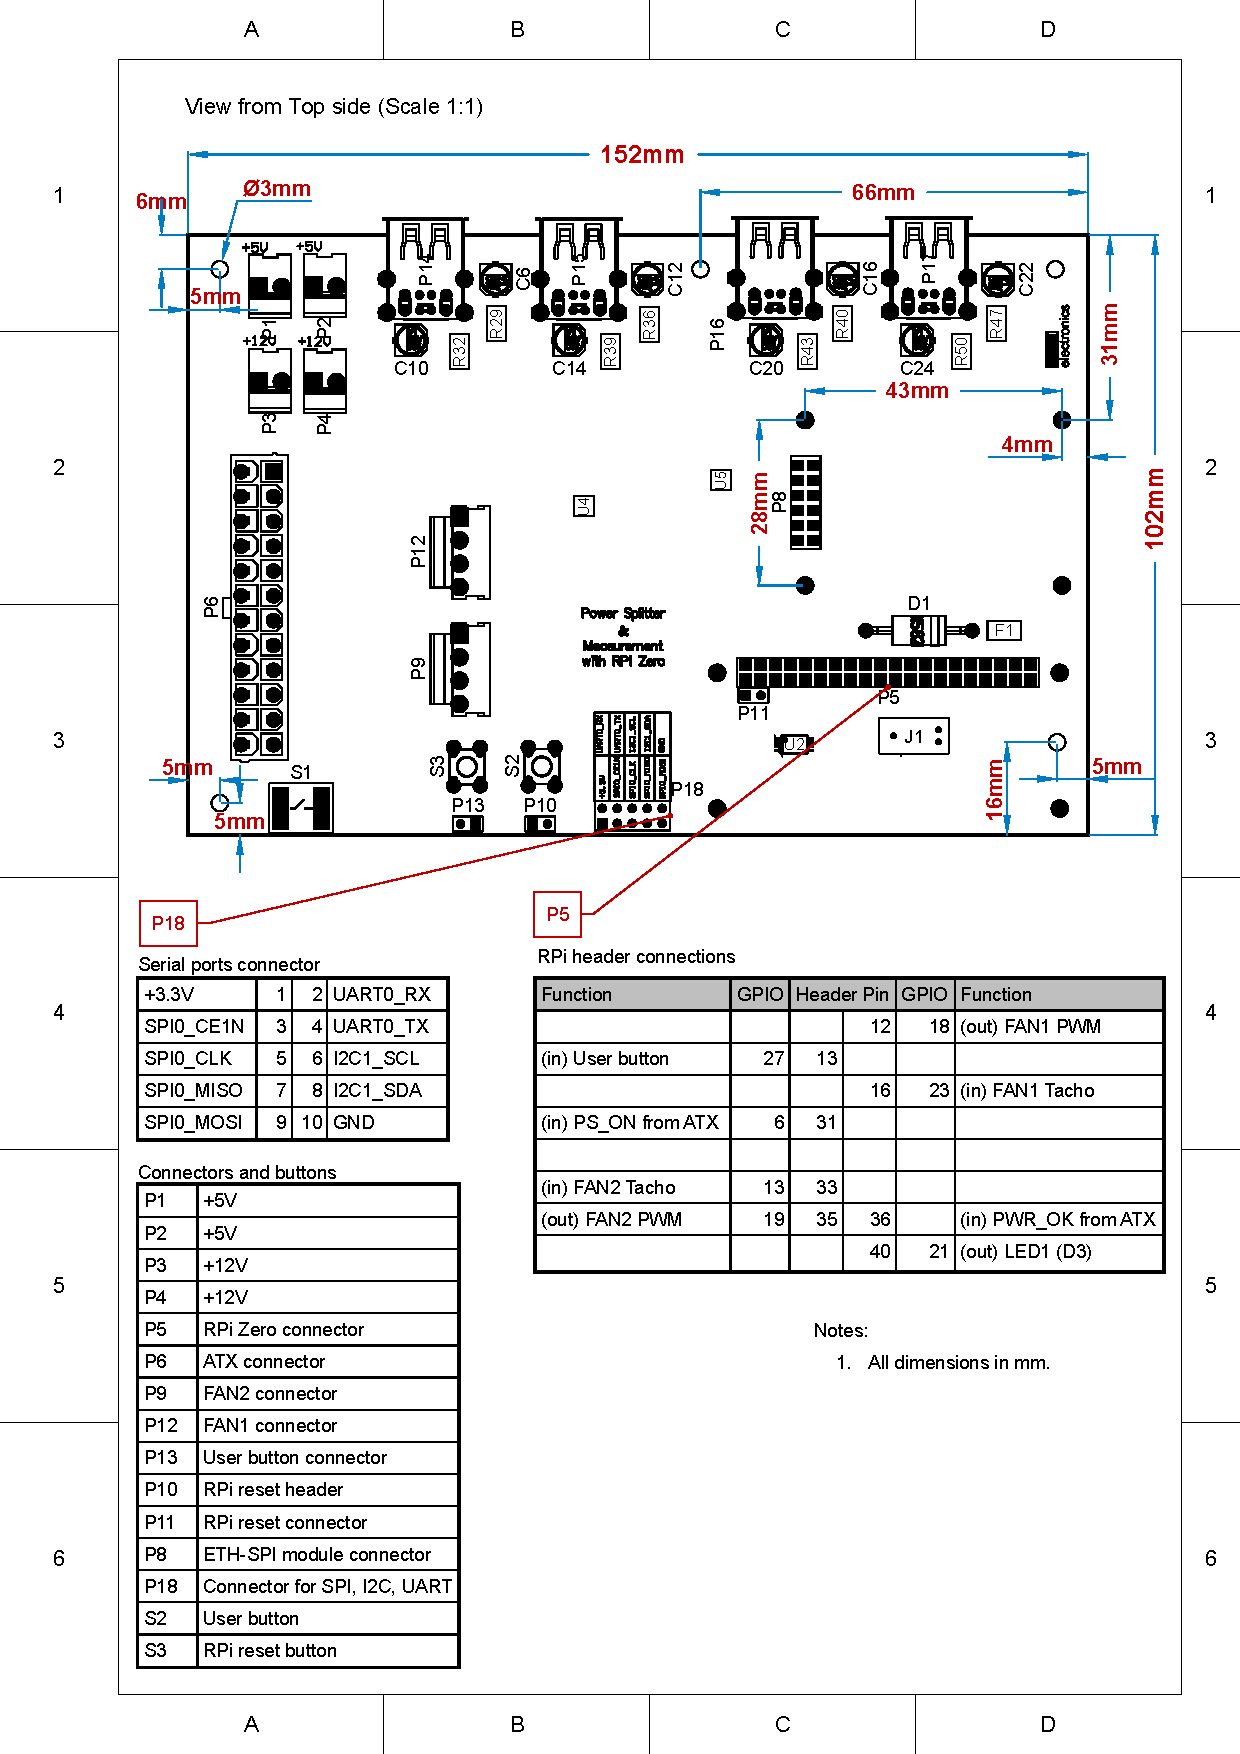
\includegraphics[
	width=\textwidth,
	height=\textheight,
	keepaspectratio
]{Drawing.pdf}
\vfill
%%\newpage
\end{document}




